% =============================================================================
% IRPP Project Report – Basic 2D Particle Filter (Monte Carlo Localization)
% =============================================================================
\documentclass[12pt, a4paper]{article}

% ── Packages ─────────────────────────────────────────────────────────────────
\usepackage[utf8]{inputenc}
\usepackage[T1]{fontenc}
\usepackage{lmodern}
\usepackage[margin=1in]{geometry}
\usepackage{amsmath, amssymb, amsfonts}
\usepackage{graphicx}
\graphicspath{{figures/}}
\usepackage{float}
\usepackage{booktabs}
\usepackage{multirow}
\usepackage{enumitem}
\usepackage{hyperref}
\usepackage{xcolor}
\usepackage{algorithm}
\usepackage{algpseudocode}
\usepackage{caption}
\usepackage{subcaption}
\usepackage{tikz}
\usetikzlibrary{positioning, arrows.meta}
\usepackage{pgfplots}
\pgfplotsset{compat=1.18}
\usepackage{listings}
\usepackage{tcolorbox}

% ── Custom colours ───────────────────────────────────────────────────────────
\definecolor{placeholderBg}{RGB}{235,235,245}
\definecolor{placeholderBorder}{RGB}{100,100,180}

% ── Placeholder box command ──────────────────────────────────────────────────
\newtcolorbox{placeholder}[1][]{%
  colback=placeholderBg,
  colframe=placeholderBorder,
  fonttitle=\bfseries,
  title={#1},
  sharp corners,
  boxrule=0.8pt,
  left=6pt, right=6pt, top=4pt, bottom=4pt
}

% ── Listings style for Python / C++ ─────────────────────────────────────────
\lstset{
  basicstyle=\ttfamily\small,
  keywordstyle=\color{blue}\bfseries,
  commentstyle=\color{gray},
  stringstyle=\color{red!70!black},
  numbers=left,
  numberstyle=\tiny\color{gray},
  frame=single,
  breaklines=true,
  captionpos=b
}

% ── Title ────────────────────────────────────────────────────────────────────
\title{%
  \textbf{Basic 2D Particle Filter (Monte Carlo Localization) Node} \\[6pt]
  \large Introduction to Robotics: Perception and Planning (IRPP) 
}
\author{
  % ── PUT YOUR NAME(S) AND ROLL NUMBER(S) HERE ──
  Inesh Roy \\ 2024112015 \\
  Satvik Shrivastava \\ 2024102029 \\
  Navanshu Gupta \\ 2024102072 \\
}
\date{ECX Hell Yeah}

% =============================================================================
\begin{document}
\maketitle
\thispagestyle{empty}
\newpage
\tableofcontents
\newpage

% #############################################################################
%                        SECTION 1 – INTRODUCTION
% #############################################################################
\section{Introduction}

Localization---determining a robot's pose (position and orientation) within a known environment---is one of the most fundamental problems in mobile robotics.
Without an accurate estimate of its own pose, a robot cannot plan collision-free paths, manipulate objects, or meaningfully interact with its surroundings.

\textbf{Monte Carlo Localization (MCL)}, also known as the \textbf{Particle Filter} approach to localization, overcomes these limitations by representing the robot's belief as a set of weighted samples (\textit{particles}) drawn from the state space.  Each particle is a hypothesis about the robot's true pose.  By recursively applying a \textit{motion model} (predict step), a \textit{measurement model} (update step), and a \textit{resampling} step, the particle cloud converges from a uniform spread across the map to a tight cluster around the true robot pose.

\subsection{Problem Statement}
This involves building a particle filter to localize a robot moving in a 2D grid world with known landmarks. The robot does not know its starting position, so it scatters particles (hypotheses) across the map. As the robot moves (odometry) and senses landmarks (range/bearing sensors), particles that do not match the sensor readings are removed, and new particles are generated around the best-fitting positions. The simulation shows the particles converging on the actual robot position over time.

\begin{itemize}
    \item \textbf{Rviz Visualization:} A visualization showing the robot's path, landmarks, and particles (colored dots) converging towards the actual robot position.
    \item \textbf{Error Reduction Plot:} A plot illustrating the average error reduction over time.
    \item \textbf{Effect of Particle Number:} An explanation of how the number of particles affects the accuracy of the localization process.
    \item \textbf{Comparison to Existing MCL Package:} A comparison between the custom implementation and an existing Monte Carlo Localization (MCL) package.
\end{itemize}

% #############################################################################
%             SECTION 2 – THEORETICAL / MATHEMATICAL BACKGROUND
% #############################################################################
\section{Theoretical \& Mathematical Background}
\label{sec:theory}

% ─────────────────────────────────────────────────────────────────────────────
\subsection{Bayesian Filtering}
\label{subsec:bayes}

The particle filter is a \emph{recursive Bayesian filter}.  Let the robot's state at time \(t\) be denoted \(\mathbf{x}_t = (x_t,\, y_t,\, \theta_t)^\top\), comprising its 2-D position \((x, y)\) and heading \(\theta\).

\paragraph{Belief.}
The \textbf{belief} \(\text{bel}(\mathbf{x}_t)\) is the posterior probability density over the robot's state given all controls \(\mathbf{u}_{1:t}\) and observations \(\mathbf{z}_{1:t}\):
\begin{equation}
  \text{bel}(\mathbf{x}_t) = p(\mathbf{x}_t \mid \mathbf{z}_{1:t},\, \mathbf{u}_{1:t}).
  \label{eq:belief}
\end{equation}

\paragraph{Prediction (Chapman–Kolmogorov).}
Incorporating the latest control \(\mathbf{u}_t\) yields the \textit{predicted belief} (also called the \textit{prior}):
\begin{equation}
  \overline{\text{bel}}(\mathbf{x}_t)
    = \int p(\mathbf{x}_t \mid \mathbf{u}_t,\, \mathbf{x}_{t-1})\;
          \text{bel}(\mathbf{x}_{t-1})\; d\mathbf{x}_{t-1}.
  \label{eq:predict}
\end{equation}
Here,
\begin{itemize}[nosep]
  \item \(p(\mathbf{x}_t \mid \mathbf{u}_t, \mathbf{x}_{t-1})\) is the \textbf{motion model} (state transition probability).
  \item The integral marginalizes over all possible previous states.
\end{itemize}

\paragraph{Update (Bayes' Rule).}
Upon receiving an observation \(\mathbf{z}_t\), the belief is corrected:
\begin{equation}
  \text{bel}(\mathbf{x}_t)
    = \eta\; p(\mathbf{z}_t \mid \mathbf{x}_t)\;
      \overline{\text{bel}}(\mathbf{x}_t),
  \label{eq:update}
\end{equation}
where
\begin{itemize}[nosep]
  \item \(p(\mathbf{z}_t \mid \mathbf{x}_t)\) is the \textbf{measurement model} (likelihood of the observation given the state).
  \item \(\eta\) is a normalization constant ensuring the belief integrates to 1.
\end{itemize}

\paragraph{The Markov Assumption.}
Equations~\eqref{eq:predict} and~\eqref{eq:update} rely on the \textbf{Markov assumption}: conditioned on \(\mathbf{x}_{t-1}\), the state \(\mathbf{x}_t\) is independent of all earlier states and observations. 

% ─────────────────────────────────────────────────────────────────────────────
\subsection{Particle Filter – Sample-Based Belief}
\label{subsec:pf}
 The \textbf{particle filter} sidesteps this by represents the belief with a finite set of \(N\) weighted samples:
\begin{equation}
  \mathcal{X}_t = \bigl\{(\mathbf{x}_t^{[i]},\; w_t^{[i]})\bigr\}_{i=1}^{N},
  \quad \sum_{i=1}^{N} w_t^{[i]} = 1.
  \label{eq:particle_set}
\end{equation}
Each particle \(\mathbf{x}_t^{[i]} = (x^{[i]}, y^{[i]}, \theta^{[i]})^\top\) is a hypothesis about the robot's pose, and \(w_t^{[i]}\) is its importance weight reflecting how well that hypothesis explains the observations.

The empirical density approximation is:
\begin{equation}
  \text{bel}(\mathbf{x}_t) \approx \sum_{i=1}^{N} w_t^{[i]}\; \delta(\mathbf{x}_t - \mathbf{x}_t^{[i]}),
  \label{eq:empirical}
\end{equation}
where \(\delta(\cdot)\) is the Dirac delta function.  As \(N \to \infty\), the approximation converges to the true posterior.

% ─────────────────────────────────────────────────────────────────────────────
\subsection{Motion Model (Predict Step)}
\label{subsec:motion}


We use the \textbf{odometry motion model} (Thrun et al., \textit{Probabilistic Robotics}).  At each step the filter receives the robot's odometry pose, and the motion since the previous pose, \((\Delta x, \Delta y, \Delta\theta)\), is decomposed into an initial rotation, a translation and a final rotation:
\begin{align}
  \delta_{\text{trans}} &= \sqrt{\Delta x^2 + \Delta y^2}, \label{eq:odom_trans} \\
  \delta_{\text{rot1}}  &= \operatorname{atan2}(\Delta y,\, \Delta x) - \theta_{t-1}, \label{eq:odom_rot1} \\
  \delta_{\text{rot2}}  &= \Delta\theta - \delta_{\text{rot1}}. \label{eq:odom_rot2}
\end{align}
If the robot only rotates (\(\delta_{\text{trans}} \approx 0\)), \(\delta_{\text{rot1}}\) is set to zero and the whole rotation goes into \(\delta_{\text{rot2}}\).  All angles are wrapped into \((-\pi, \pi]\).

\paragraph{Adding Noise.}
Real odometry is corrupted by slip, wheel encoder errors, and unmodelled terrain effects.  For every particle we add Gaussian noise to each component, with a standard deviation that grows with the size of the motion:
\begin{align}
  \hat{\delta}_{\text{rot1}}  &= \delta_{\text{rot1}}  + \mathcal{N}\bigl(0,\; \alpha_{\text{rot}} |\delta_{\text{rot1}}| + \alpha_{\text{trans}}\, \delta_{\text{trans}}\bigr), \label{eq:noise_rot1} \\
  \hat{\delta}_{\text{trans}} &= \delta_{\text{trans}} + \mathcal{N}\bigl(0,\; \alpha_{\text{trans}}\, \delta_{\text{trans}} + \alpha_{\text{rot}} |\Delta\theta|\bigr), \label{eq:noise_trans} \\
  \hat{\delta}_{\text{rot2}}  &= \delta_{\text{rot2}}  + \mathcal{N}\bigl(0,\; \alpha_{\text{rot}} |\delta_{\text{rot2}}| + \alpha_{\text{trans}}\, \delta_{\text{trans}}\bigr), \label{eq:noise_rot2}
\end{align}
with \(\alpha_{\text{rot}} = 0.05\) and \(\alpha_{\text{trans}} = 0.02\).  A small constant (\(10^{-4}\)) is added to each standard deviation so that the particles keep spreading slightly even when the robot is still.

\paragraph{Predict Step (per particle).}
For every particle \(i\):
\begin{enumerate}[nosep]
  \item Decompose the observed motion into \(\delta_{\text{rot1}}, \delta_{\text{trans}}, \delta_{\text{rot2}}\) (Eqs.~\eqref{eq:odom_trans}--\eqref{eq:odom_rot2}).
  \item Add Gaussian noise to each component (Eqs.~\eqref{eq:noise_rot1}--\eqref{eq:noise_rot2}).
  \item Propagate the particle:
  \begin{align}
    \theta' &= \theta^{[i]} + \hat{\delta}_{\text{rot1}}, \label{eq:prop_rot1} \\
    x^{[i]} &\gets x^{[i]} + \hat{\delta}_{\text{trans}} \cos\theta', \qquad
    y^{[i]} \gets y^{[i]} + \hat{\delta}_{\text{trans}} \sin\theta', \label{eq:prop_xy} \\
    \theta^{[i]} &\gets \theta' + \hat{\delta}_{\text{rot2}}. \label{eq:prop_rot2}
  \end{align}
  \item If the particle has moved into an obstacle or off the map, it is replaced by a random pose in free space.
\end{enumerate}
This is equivalent to sampling from \(p(\mathbf{x}_t \mid \mathbf{u}_t, \mathbf{x}_{t-1}^{[i]})\), thereby implementing Eq.~\eqref{eq:predict} via Monte Carlo sampling.

% ─────────────────────────────────────────────────────────────────────────────
\subsection{Measurement Model (Update Step)}
\label{subsec:measurement}

The robot is equipped with a \textbf{range-bearing sensor} that can detect landmarks within a maximum range \(r_{\max}\).  For a landmark \(l_j\) located at \((l_{j,x},\, l_{j,y})\) and a particle at \((x^{[i]}, y^{[i]}, \theta^{[i]})\), the expected measurement is:
\begin{align}
  \hat{r}_j^{[i]}   &= \sqrt{(l_{j,x} - x^{[i]})^2 + (l_{j,y} - y^{[i]})^2}, \label{eq:exp_range} \\
  \hat{\phi}_j^{[i]} &= \operatorname{atan2}\!\bigl(l_{j,y} - y^{[i]},\; l_{j,x} - x^{[i]}\bigr) - \theta^{[i]}. \label{eq:exp_bearing}
\end{align}

The actual sensor returns a noisy measurement \(\mathbf{z}_j = (r_j, \phi_j)^\top\).  We model the noise as independent Gaussians:
\begin{equation}
  p(\mathbf{z}_j \mid \mathbf{x}^{[i]}, l_j)
    = \frac{1}{2\pi\,\sigma_r\,\sigma_\phi}\;
      \exp\!\Biggl(
        -\frac{(r_j - \hat{r}_j^{[i]})^2}{2\sigma_r^2}
        -\frac{(\phi_j - \hat{\phi}_j^{[i]})^2}{2\sigma_\phi^2}
      \Biggr),
  \label{eq:meas_likelihood}
\end{equation}
where \(\sigma_r\) and \(\sigma_\phi\) are the standard deviations of range and bearing noise respectively.  The simulated sensor has a range of \(r_{\max} = 8\) m and noise of 0.2 m in range and 0.05 rad in bearing.  The filter uses slightly larger values, \(\sigma_r = 0.3\) m and \(\sigma_\phi = 0.1\) rad, so that it is not over-confident.  Each reading carries the index of the landmark it belongs to, so the data association between measurements and landmarks is known.

\paragraph{Importance Weight.}
If \(K\) landmarks are observed at time \(t\), the weight of particle \(i\) is updated as:
\begin{equation}
  w_t^{[i]} = w_{t-1}^{[i]} \prod_{j=1}^{K} p(\mathbf{z}_j \mid \mathbf{x}_t^{[i]}, l_j).
  \label{eq:weight}
\end{equation}
After computing all weights, they are normalized:
\begin{equation}
  \tilde{w}_t^{[i]} = \frac{w_t^{[i]}}{\sum_{k=1}^{N} w_t^{[k]}}.
  \label{eq:normalize}
\end{equation}
The normalization constant \(\eta = 1 / \sum_k w_t^{[k]}\) corresponds to the \(\eta\) in Eq.~\eqref{eq:update}.

\paragraph{Handling Bearing Wrap-Around.}
When computing the bearing difference \(\phi_j - \hat{\phi}_j^{[i]}\), the result must be wrapped into \((-\pi, \pi]\) to avoid discontinuities:
\begin{equation}
  \Delta\phi = \operatorname{atan2}\!\bigl(\sin(\phi_j - \hat{\phi}_j^{[i]}),\; \cos(\phi_j - \hat{\phi}_j^{[i]})\bigr).
  \label{eq:wrap}
\end{equation}
% ─────────────────────────────────────────────────────────────────────────────
\subsection{Resampling}
\label{subsec:resample}

After several update steps, the weight distribution typically becomes skewed: a few particles carry most of the probability mass while the rest have negligible weights.  This \textit{particle degeneracy} problem is addressed by \textbf{resampling}: drawing a new set of particles from the current set with replacement, where the probability of selecting particle \(i\) is proportional to \(\tilde{w}_t^{[i]}\).  In our implementation, resampling is performed \textbf{at every update step} to keep the particle cloud responsive.

\subsubsection{Low-Variance (Systematic) Resampling}
We employ the \textbf{low-variance resampling} algorithm, which is both efficient (\(O(N)\)) and introduces less sampling variance than multinomial resampling.

\begin{algorithm}[H]
\caption{Low-Variance Resampling}
\label{alg:resample}
\begin{algorithmic}[1]
\Require Particle set $\mathcal{X} = \{(\mathbf{x}^{[i]}, \tilde{w}^{[i]})\}_{i=1}^{N}$
\Ensure  New particle set $\mathcal{X}'$ with uniform weights
\State $r \sim \mathcal{U}(0, 1/N)$ \Comment{single random draw}
\State $c \gets \tilde{w}^{[1]}$
\State $j \gets 1$
\For{$i = 1$ \textbf{to} $N$}
  \State $U \gets r + (i - 1) / N$
  \While{$U > c$}
    \State $j \gets j + 1$
    \State $c \gets c + \tilde{w}^{[j]}$
  \EndWhile
  \State Add $(\mathbf{x}^{[j]},\; 1/N)$ to $\mathcal{X}'$
\EndFor
\State \Return $\mathcal{X}'$
\end{algorithmic}
\end{algorithm}

The key insight is that a single random number \(r\) generates \(N\) evenly spaced thresholds \(\{r, r+1/N, r+2/N, \ldots\}\) that ``sweep'' across the cumulative weight distribution.  This ensures that particles with high weights are selected proportionally without the high variance of independent draws.

\subsubsection{Particle Deprivation and Recovery}
After many resampling steps, particles may lose diversity and collapse to a single mode.  This is the \textit{particle deprivation} problem.  Our implementation uses two mitigations:
\begin{enumerate}[nosep]
  \item \textbf{Random particle injection:} At every resampling step, 15\% of the particle budget is replaced with particles drawn uniformly from free space, ensuring continuous exploration.
  \item \textbf{Lost detection:} If the largest unnormalized particle weight stays below \(w_{\min} = 10^{-50}\) for 8 consecutive updates, the filter declares the robot lost and reinitialises all particles globally.
\end{enumerate}

% ─────────────────────────────────────────────────────────────────────────────
\subsection{Complete MCL Algorithm}
\label{subsec:mcl_algo}
The following summarises the full MCL loop.

\begin{algorithm}[H]
\caption{Monte Carlo Localization (MCL)}
\label{alg:mcl}
\begin{algorithmic}[1]
\Require Occupancy grid map $\mathcal{M}$ (for free space), landmark positions $\{l_j\}$,\; particle count $N = 500$
\State \textbf{Initialization:} Sample $\mathcal{X}_0 = \{\mathbf{x}_0^{[i]}\}_{i=1}^{N}$ uniformly over free space; set $w_0^{[i]} = 1/N$
\For{each time step $t = 1, 2, \ldots$}
  \State Receive odometry displacement $(\Delta x, \Delta y, \Delta\theta)$ and landmark readings $\{\mathbf{z}_j\}$
  \For{$i = 1$ \textbf{to} $N$} \Comment{\textsc{Predict}}
    \State Decompose displacement and add noise (Eqs.~\eqref{eq:odom_trans}--\eqref{eq:noise_rot2})
    \State Propagate particle (Eqs.~\eqref{eq:prop_rot1}--\eqref{eq:prop_rot2})
  \EndFor
  \For{$i = 1$ \textbf{to} $N$} \Comment{\textsc{Update}}
    \State Compute the expected range and bearing to each observed landmark (Eqs.~\eqref{eq:exp_range}--\eqref{eq:exp_bearing})
    \State Compute $w_t^{[i]}$ from the measurement likelihood (Eqs.~\eqref{eq:meas_likelihood}--\eqref{eq:weight})
  \EndFor
  \State Normalize weights: $\tilde{w}_t^{[i]} \gets w_t^{[i]} / \sum_k w_t^{[k]}$
  \State $\mathcal{X}_t \gets$ \Call{LowVarianceResample}{$\mathcal{X}_t$} with 15\% random injection \Comment{\textsc{Resample}}
  \If{$\max_i \tilde{w}_t^{[i]} < w_{\min}$ for $T$ consecutive steps} \Comment{\textsc{Lost Detection}}
    \State Reinitialise all particles globally
  \EndIf
\EndFor
\end{algorithmic}
\end{algorithm}

% ─────────────────────────────────────────────────────────────────────────────
\subsection{Convergence and Particle Count}
\label{subsec:convergence}

The accuracy of a particle filter depends on the number of particles \(N\):
 Increasing \(N\) improves the approximation of the true posterior distribution, reducing localization error.
The computational cost of each iteration grows linearly with \(N\).
  Too few particles may cause filter divergence, while too many particles reduce real-time performance.
In our implementation, we use a fixed particle count of \(N = 500\); Section~\ref{subsec:particles} shows how the filter behaves with fewer and more particles.







% #############################################################################
%             SECTION 3 – IMPLEMENTATION
% #############################################################################
\section{Implementation}
\label{sec:implementation}

This section describes the software architecture and the from-scratch implementation of each MCL step as a ROS~2 node written in Python.  Each node runs in its own Docker container (ROS~2 Humble), started together with Docker Compose.

% ─────────────────────────────────────────────────────────────────────────────
\subsection{System Overview}
The implementation consists of the following components:
\begin{enumerate}[nosep]
  \item \textbf{Map server} (\texttt{nav2\_map\_server}) -- publishes the occupancy grid of the 20\,m \(\times\) 20\,m world (0.05\,m per cell).
  \item \textbf{Simulated robot} -- drives around the map on its own while avoiding walls, publishes its ground-truth pose, and simulates the range-bearing sensor for 5 landmarks.  Every 30\,s it is teleported to a random free pose (the kidnapped robot problem).
  \item \textbf{Custom MCL node} -- subscribes to odometry and landmark readings, runs the particle filter, and publishes the estimated pose, its confidence (the largest particle weight) and the particle cloud.
  \item \textbf{Scan bridge} -- turns the robot's motion into odometry for both filters, and produces what \texttt{nav2\_amcl} needs: a simulated 36-beam laser scan (ray-cast on the map) and the odometry transform.  When it detects a kidnap, it asks AMCL to relocalize globally.
  \item \textbf{Nav2 AMCL} -- the existing MCL package used for comparison (Section~\ref{sec:comparison}).
  \item \textbf{RViz, live plots and results logger} -- visualize the robot, landmarks and both particle clouds, plot the error of both filters, and save the errors to CSV files.
\end{enumerate}

\begin{figure}[H]
    \centering
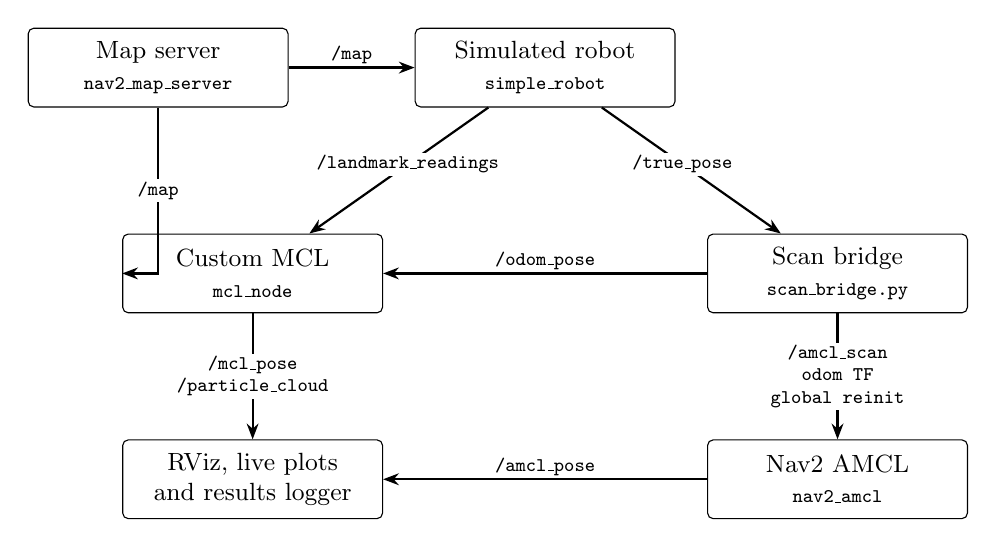
\begin{tikzpicture}[
    node distance=1.2cm and 1.6cm,
    box/.style={draw, rounded corners=2pt, align=center, minimum width=3.3cm, minimum height=1.0cm, font=\small},
    topic/.style={font=\scriptsize\ttfamily, fill=white, inner sep=1pt},
    arr/.style={-{Stealth[length=2mm]}, thick}
  ]
  \node[box] (robot) {Simulated robot\\\scriptsize\texttt{simple\_robot}};
  \node[box, below left=1.6cm and 0.4cm of robot] (mcl) {Custom MCL\\\scriptsize\texttt{mcl\_node}};
  \node[box, below right=1.6cm and 0.4cm of robot] (bridge) {Scan bridge\\\scriptsize\texttt{scan\_bridge.py}};
  \node[box, below=1.6cm of bridge] (amcl) {Nav2 AMCL\\\scriptsize\texttt{nav2\_amcl}};
  \node[box, below=1.6cm of mcl] (viz) {RViz, live plots\\and results logger};
  \node[box, left=1.6cm of robot] (map) {Map server\\\scriptsize\texttt{nav2\_map\_server}};

  \draw[arr] (robot) -- node[topic, pos=0.45] {/landmark\_readings} (mcl);
  \draw[arr] (robot) -- node[topic, pos=0.45] {/true\_pose} (bridge);
  \draw[arr] (bridge.west) -- node[topic, above] {/odom\_pose} (mcl.east);
  \draw[arr] (bridge) -- node[topic, align=center] {/amcl\_scan\\odom TF\\global reinit} (amcl);
  \draw[arr] (mcl) -- node[topic, align=center] {/mcl\_pose\\/particle\_cloud} (viz);
  \draw[arr] (amcl.west) -- node[topic, above] {/amcl\_pose} (viz.east);
  \draw[arr] (map) |- node[topic, pos=0.25] {/map} (mcl.west);
  \draw[arr] (map) -- node[topic, above] {/map} (robot);
\end{tikzpicture}
    \caption{ROS~2 node communication graph.  \texttt{/map} also goes to the scan bridge, AMCL and RViz, and \texttt{/true\_pose} also goes to the plots and the results logger.}
    \label{fig:architecture}
\end{figure}

\subsection{Test Maps}
\label{subsec:maps}
Figure~\ref{fig:maps} shows the maps used in the experiments.  The five landmarks are at the same positions on every map; they are treated as point beacons, so they may lie inside obstacles.  Map~1 is symmetric under a 180\textdegree{} rotation and Map~2 under 90\textdegree{} rotations.  Map~4 is Map~1 with two extra obstacles that remove the symmetry.  The symmetry does not matter for our filter, which knows which landmark each reading belongs to, but it matters for AMCL, which only sees a laser scan (Section~\ref{subsec:symmetry}).

\begin{figure}[H]
    \centering
    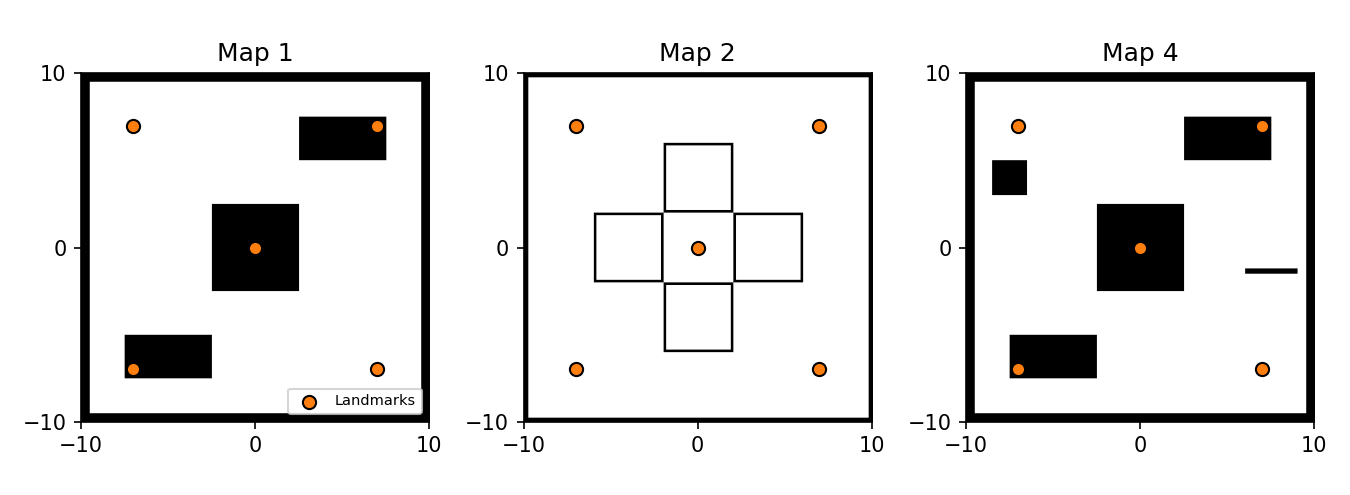
\includegraphics[width=\textwidth]{maps.png}
    \caption{The maps used in the experiments, with the landmark positions.  Each map is 20\,m \(\times\) 20\,m.}
    \label{fig:maps}
\end{figure}

% ─────────────────────────────────────────────────────────────────────────────


% #############################################################################
%             SECTION 4 – RESULTS
% #############################################################################
\section{Results}
\label{sec:results}

% ─────────────────────────────────────────────────────────────────────────────
\subsection{RViz Visualization}

The following screenshots from RViz show the custom MCL running on Map~1 and Map~2 after it has converged.  The particles are shown as red dots: most of them form a tight cluster at the robot (the cyan marker), and the scattered dots are the 15\% random particles injected at every resampling step.  The blue arrow is the MCL pose estimate.

\begin{figure}[H]
    \centering
    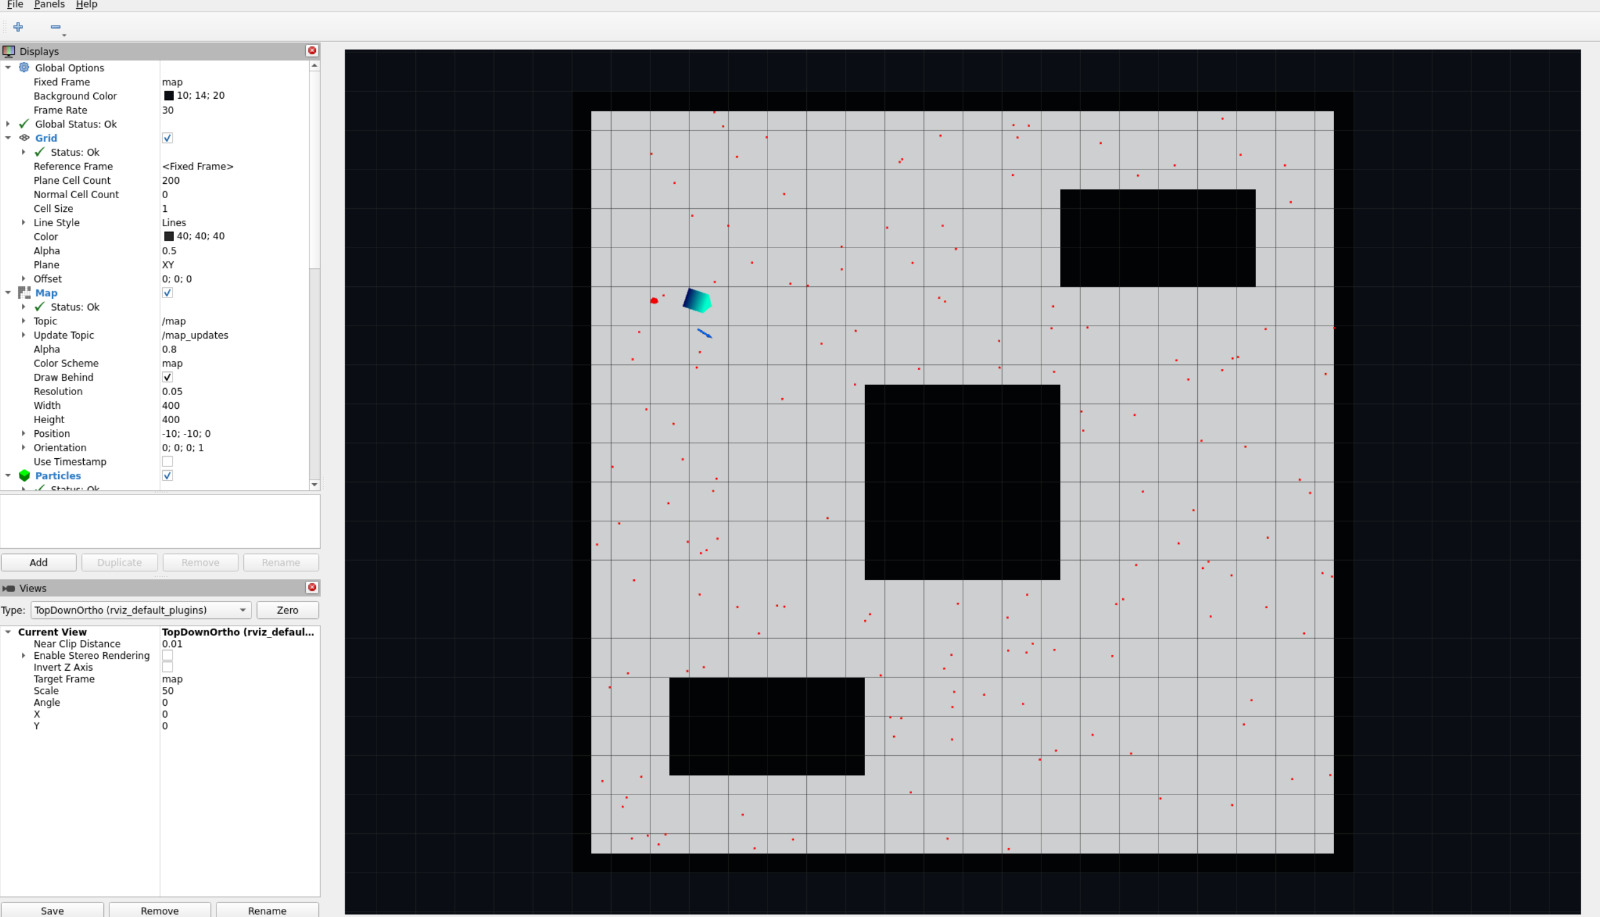
\includegraphics[width=0.9\textwidth]{map1_4.1.png}
    \caption{RViz visualization for Map~1}
\end{figure}

\begin{figure}[H]
    \centering
    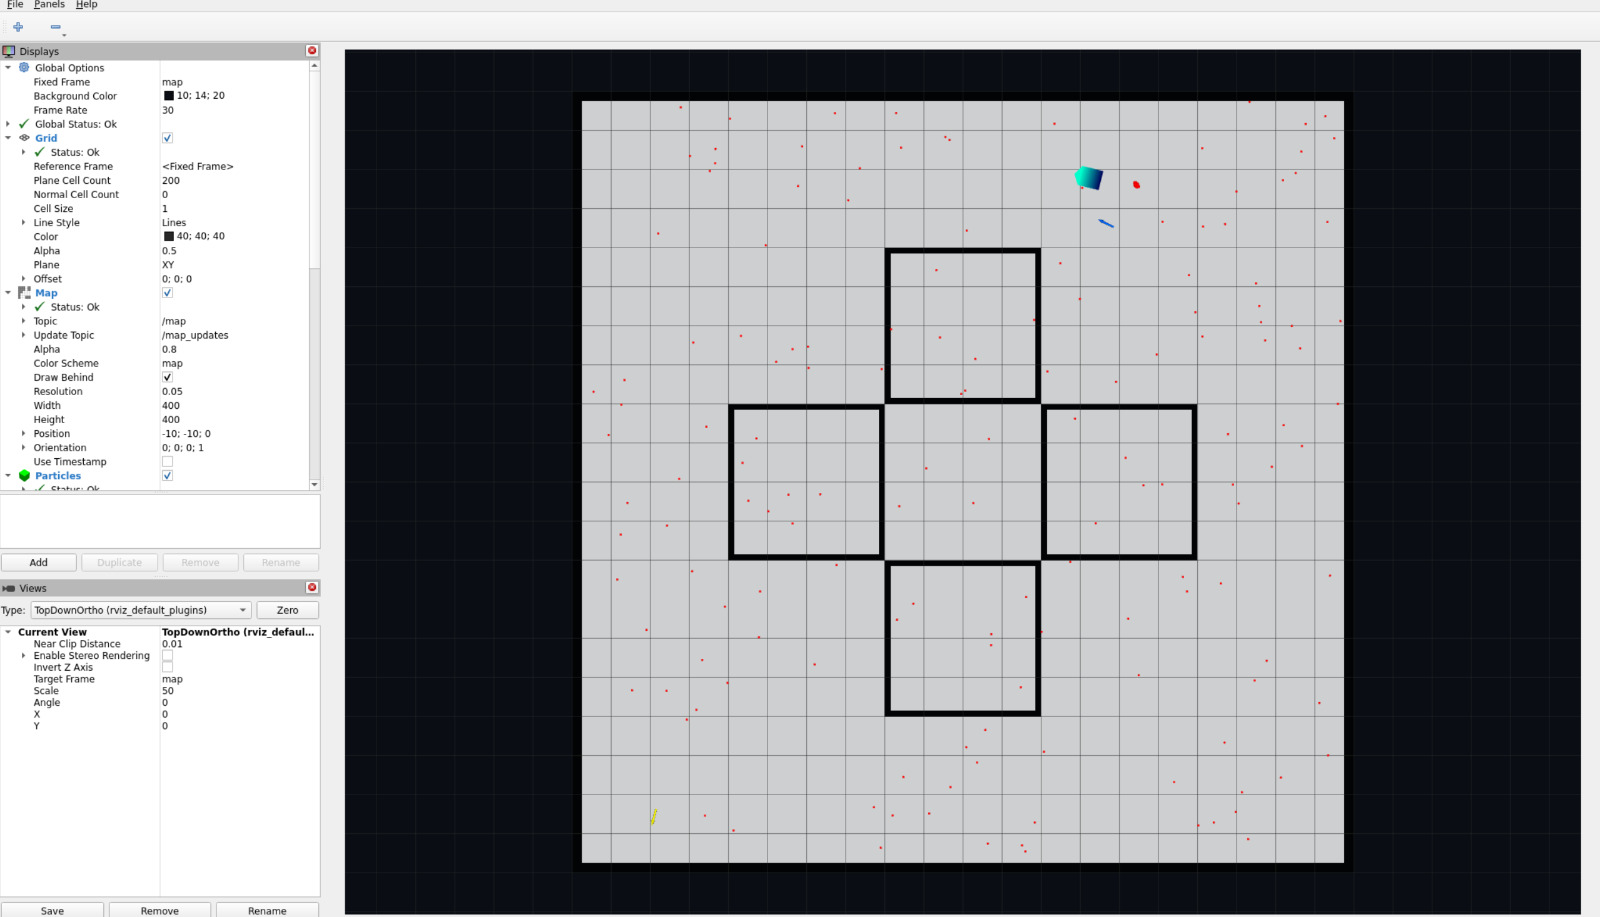
\includegraphics[width=0.9\textwidth]{map2_4.1.png}
    \caption{RViz visualization for Map~2}
\end{figure}

% ─────────────────────────────────────────────────────────────────────────────
\subsection{Localization Error Over Time}

The localization error at time \(t\) is defined as the Euclidean distance between the estimated pose and the ground-truth pose:
\begin{equation}
  e_t = \sqrt{(\hat{x}_t - x_t^*)^2 + (\hat{y}_t - y_t^*)^2},
  \label{eq:error}
\end{equation}
where \((x_t^*, y_t^*)\) is the ground-truth position.

Figure~\ref{fig:error} shows the error of the custom MCL over a 330\,s run on Map~1 and on Map~2.  At the start the particles are spread over the whole map and the error is about 8--9\,m.  In this run the filter converged to within 1\,m in 6.1\,s on Map~1 and 6.6\,s on Map~2.

\begin{figure}[H]
    \centering
    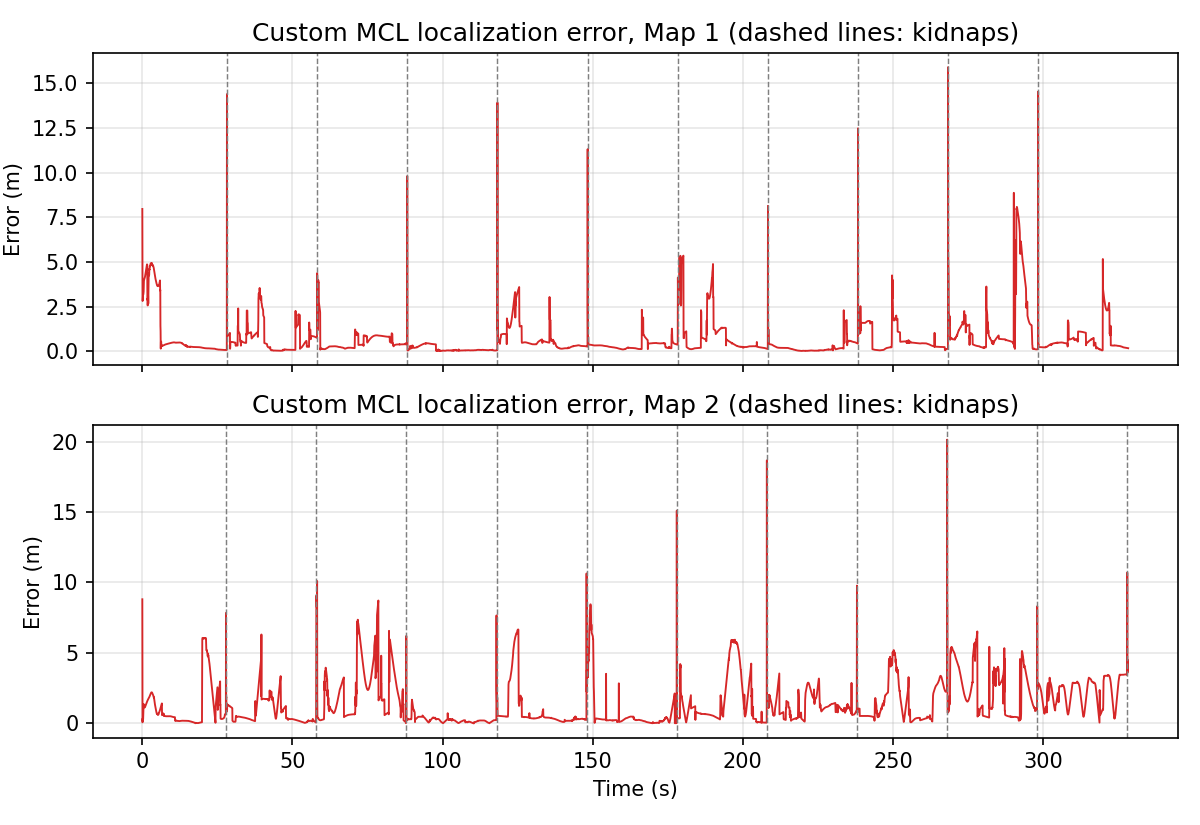
\includegraphics[width=\textwidth]{error_custom_mcl.png}
    \caption{Localization error of the custom MCL over time on Map~1 and Map~2.  The dashed lines mark the kidnaps.}
    \label{fig:error}
\end{figure}

The large spikes at the dashed lines happen every 30\,s, when the robot is teleported to a random position on the map (the kidnapped robot problem).  At that moment the particles are still at the old position, so the error jumps to the distance of the teleport.  The particles that are injected at random then land near the new position, receive high weights, and the cloud re-forms there.  The smaller spikes between kidnaps happen in parts of the map where only one or two landmarks are within the 8\,m sensor range, for example near the corners: with a single landmark the range and bearing only constrain the robot to a circle around it, so the estimate can drift until more landmarks come into view.

We measure the recovery after each kidnap as the time until the error stays below 1\,m for 3\,s, and count a kidnap as recovered if the median error over the last 10\,s before the next kidnap is below 1\,m.  Over two such runs per map (20 kidnaps each), the filter recovered from 17 of 20 kidnaps on Map~1 (median recovery time 2.8\,s) and from 15 of 20 on Map~2 (median 2.3\,s).  After recovering, the median error was 0.29\,m on Map~1 and 0.40\,m on Map~2.  The larger error on Map~2 comes from periods in which the estimate is off by 2--5\,m for several seconds, for example after 240\,s in Figure~\ref{fig:error}.

% ─────────────────────────────────────────────────────────────────────────────
% ─────────────────────────────────────────────────────────────────────────────
\subsection{Effect of the Number of Particles}
\label{subsec:particles}
To see how the number of particles affects the filter, we ran it on Map~4 with \(N \in \{50, 100, 250, 500, 1000\}\), twice for 230\,s each, which gives 12 complete kidnaps per value.  Figure~\ref{fig:particles} shows the share of kidnaps the filter recovered from and the error after recovery.

\begin{figure}[H]
    \centering
    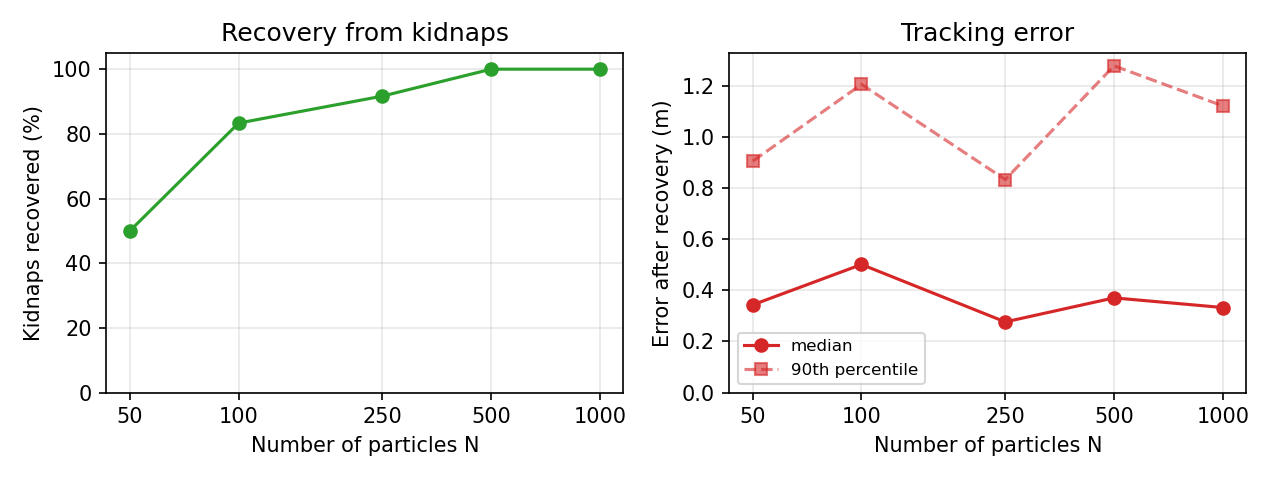
\includegraphics[width=\textwidth]{particle_count.png}
    \caption{Effect of the number of particles on Map~4, over 12 kidnaps per value of \(N\).  Left: share of kidnaps after which the filter re-localized.  Right: error after recovery.}
    \label{fig:particles}
\end{figure}

The number of particles mainly affects \textbf{whether} the filter recovers from a kidnap.  With \(N = 50\) it recovered from only 6 of 12 kidnaps, with 100 from 10 of 12 and with 250 from 11 of 12; with 500 and 1000 it recovered every time.  After a kidnap, the filter can only re-localize if some of the randomly injected particles (15\% of \(N\), so only 7 when \(N = 50\)) land close to the new position.  With few particles this often does not happen before the existing cloud has locked onto a wrong position.

Once the filter had recovered, the tracking error did not depend on \(N\) in any consistent way: the median stayed between 0.28 and 0.50\,m for all values, and the recovery time between 1 and 4\,s.  The accuracy is limited by the measurements rather than by the number of samples: with only a few landmarks within 8\,m, and range noise of 0.2\,m, more particles do not give a better estimate of the pose.  The Python node kept up with the 20\,Hz odometry rate for all values of \(N\).  We therefore use \(N = 500\), the smallest value that recovered from every kidnap in this test.

% #############################################################################
%       SECTION 5 – COMPARISON WITH EXISTING MCL PACKAGE
% #############################################################################
\section{Comparison with Existing MCL Package}
\label{sec:comparison}

We compare our from-scratch implementation against the widely-used \texttt{nav2\_amcl} (Adaptive Monte Carlo Localization) package from the ROS~2 Navigation2 stack. 

\subsection{Overview of \texttt{nav2\_amcl}}
The \texttt{nav2\_amcl} package implements an adaptive variant of MCL that uses:
\begin{itemize}[nosep]
  \item \textbf{KLD-sampling} to dynamically adjust the number of particles based on the complexity of the posterior distribution.
  \item \textbf{Likelihood field} or \textbf{beam} sensor models for laser range finders instead of landmark-based measurements.
  \item \textbf{Augmented MCL} to handle the kidnapped robot problem by injecting random particles when the average observation likelihood is low.
  \item An occupancy-grid map instead of a landmark-based map.
  \item \href{https://github.com/ros-planning/navigation2/tree/humble/nav2_amcl}{nav2\_amcl GitHub Repository link}
\end{itemize}

\subsection{Feature Comparison}

\begin{table}[H]
\centering
\caption{Feature comparison between our implementation and \texttt{nav2\_amcl}.}
\label{tab:comparison}
\small
\resizebox{\textwidth}{!}{%
\begin{tabular}{@{}lll@{}}
\toprule
\textbf{Feature} & \textbf{Our Implementation} & \textbf{nav2\_amcl} \\
\midrule
Motion model    & Odometry (rot1-trans-rot2)          & Odometry (differential drive) \\
Sensor model    & Range-bearing to known landmarks    & Likelihood field (36-beam laser) \\
Map             & Landmark positions (+ grid for free space) & Occupancy grid \\
Particle count  & Fixed, $N = 500$                    & KLD-sampling, 500--20\,000 \\
Resampling      & Low-variance, every update          & Low-variance, every update \\
Kidnapped robot & 15\% random injection + lost detection & Random injection + global re-initialisation \\
Implementation  & Python                              & C++ \\
\bottomrule
\end{tabular}%
}
\end{table}

\subsection{Experimental Setup}
Both filters run at the same time on the same simulated robot and map, and receive the same odometry.  The custom MCL uses the landmark readings; AMCL uses a 36-beam laser scan that the scan bridge ray-casts on the map from the robot's true pose (range 15\,m).  AMCL is started with a global (uniform) initialisation.  When the scan bridge sees the true pose jump, it calls AMCL's \texttt{reinitialize\_global\_localization} service, which spreads the particles over the whole map again.  This gives AMCL a hint that our filter does not get: the custom MCL is not told about kidnaps and has to detect them through its own weights.

AMCL needs many particles to relocalize from a uniform spread over a 20\,m \(\times\) 20\,m map.  With at most 1000 particles, it almost never converged again after a kidnap (its error stayed at 7--9\,m), so we allow up to 20\,000; KLD-sampling reduces the count towards the minimum of 500 once the filter has converged.

We ran each of Map~1, Map~2 and Map~4 twice for 330\,s, which gives 20 kidnaps per map, and recorded the true pose and both estimates.  Recovery time and success are measured as in Section~\ref{sec:results}.  In addition, when AMCL did not recover, we checked whether its estimate was within 0.5\,m of a rotated copy of the true pose (180\textdegree{} for Map~1, 90\textdegree{}, 180\textdegree{} or 270\textdegree{} for Map~2).

\subsection{Results}

\begin{table}[H]
    \centering
    \caption{Kidnap recovery over 20 kidnaps per map (two 330\,s runs).  Recovery time is the median over the recovered kidnaps.  Tracking error is the error after recovery, given as the median and the 10th--90th percentile range.  The one AMCL kidnap on Map~2 that is in neither row ended at a pose that was neither correct nor a rotated copy.}
    \label{tab:results}
    \small
    \resizebox{\textwidth}{!}{%
\begin{tabular}{@{}llccc@{}}
        \toprule
        & & \textbf{Map 1} & \textbf{Map 2} & \textbf{Map 4} \\
        \midrule
        \multirow{3}{*}{Custom MCL}
          & Recovered            & 17 / 20 & 15 / 20 & 19 / 20 \\
          & Recovery time        & 2.8\,s & 2.3\,s & 0.7\,s \\
          & Tracking error       & 0.29\,m (0.05--0.96) & 0.40\,m (0.08--2.01) & 0.25\,m (0.06--1.19) \\
        \midrule
        \multirow{4}{*}{Nav2 AMCL}
          & Recovered            & 11 / 20 & 5 / 20 & 19 / 20 \\
          & Converged to a rotated twin & 9 / 20 & 14 / 20 & 1 / 20 \\
          & Recovery time        & 7.3\,s & 16.3\,s & 5.4\,s \\
          & Tracking error       & 0.06\,m (0.02--0.13) & 0.06\,m (0.03--0.13) & 0.06\,m (0.02--0.14) \\
        \bottomrule
    \end{tabular}%
}
\end{table}

Figure~\ref{fig:compare_map4} shows both filters on Map~4, which has no symmetry.  Here AMCL recovered from 19 of 20 kidnaps (median 5.4\,s) and then tracked the robot to within about 6\,cm.  In the remaining kidnap it settled on a rotated copy of the true pose, probably because the two extra obstacles are not visible from everywhere (the central block can hide them), so from some places the map still looks symmetric to the laser.  Our filter recovered faster (median 0.7\,s) because the landmark readings identify the robot's position directly, but it tracked less precisely, with a median error of 0.25\,m.  AMCL compares 36 laser beams against the whole map, while our filter only has the few landmarks that are within 8\,m.  At the start of the six runs, our filter converged from the uniform spread in 3.4--6.6\,s and AMCL in 4.2--11.3\,s.

\begin{figure}[H]
    \centering
    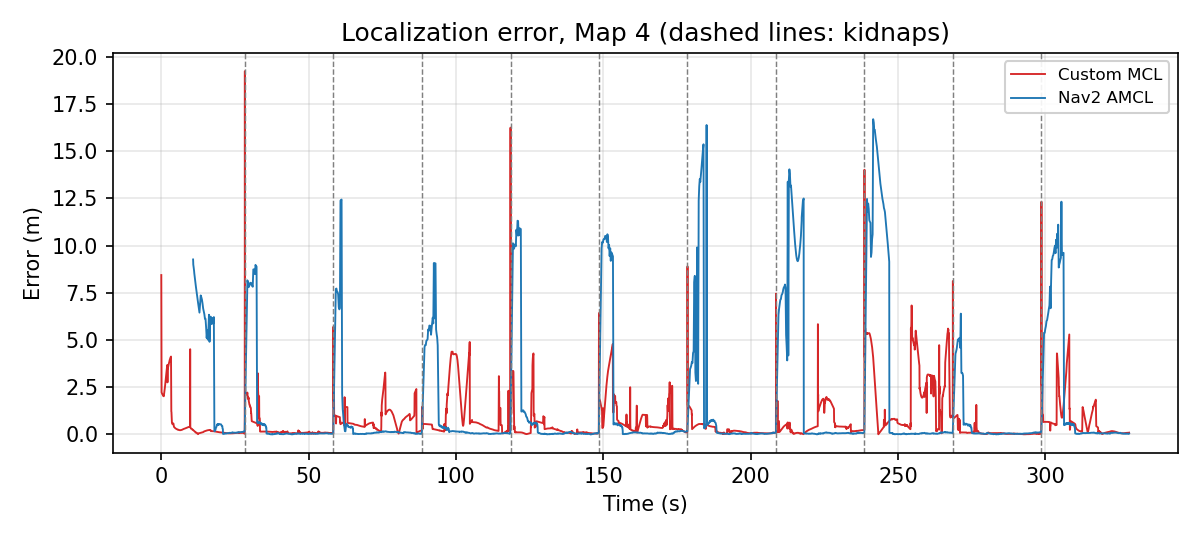
\includegraphics[width=\textwidth]{compare_map4.png}
    \caption{Localization error of both filters on Map~4.}
    \label{fig:compare_map4}
\end{figure}

\subsection{Effect of Map Symmetry}
\label{subsec:symmetry}
On the symmetric maps, AMCL often settled on the wrong pose after a kidnap: on Map~1 in 9 of 20 kidnaps and on Map~2 in 14 of 20.  In all of these cases its estimate was within 0.5\,m of a rotated copy of the true pose; only once (on Map~2) did it end up somewhere else.  On Map~1, a laser scan taken at \((x, y, \theta)\) is identical to one taken at \((-x, -y, \theta + \pi)\), so the two poses explain the measurements equally well and the filter has no way of choosing between them.  Figure~\ref{fig:compare_map1} shows this: whenever AMCL's error is large, its distance to the mirrored pose \((-x, -y)\) is close to zero.  AMCL then either tracks the mirrored pose accurately until the next kidnap or switches back and forth between the two poses (the vertical jumps in the figure).  Its random particle injection does not resolve the ambiguity, because the wrong pose fits the scans as well as the right one.

\begin{figure}[H]
    \centering
    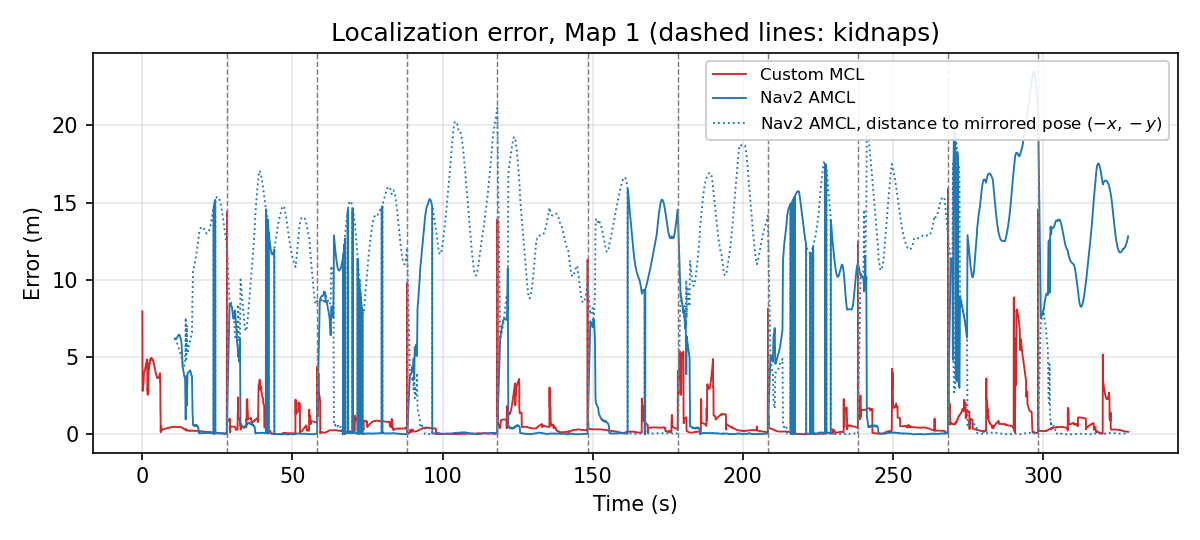
\includegraphics[width=\textwidth]{compare_map1.png}
    \caption{Localization error of both filters on Map~1.  The dotted line is the distance from AMCL's estimate to the mirrored pose \((-x, -y)\) of the robot.}
    \label{fig:compare_map1}
\end{figure}

Our filter does not have this problem, even though the landmarks themselves are placed symmetrically, because every reading carries the index of the landmark it belongs to.  This known data association is what removes the ambiguity, and it is the main advantage of the landmark-based approach in this comparison.  With a laser alone, the map itself has to be asymmetric, as in Map~4.

% #############################################################################
%             SECTION 6 – CONCLUSION & FUTURE WORK
% #############################################################################
\section{Conclusion}
\label{sec:conclusion}

\subsection{Summary}
In this project, we implemented a particle filter for Monte Carlo Localization entirely from scratch.  The three core steps---predict (motion model with Gaussian noise), update (range-bearing measurement likelihood), and resample (low-variance resampling)---were implemented as a ROS~2 Python node and validated in a 2D grid world with known landmarks.
\subsection{Key Findings}

\begin{itemize}
  \item \textbf{Global localization:} Starting with particles spread over the whole map (initial error about 8--9\,m), the filter converged to within 1\,m in 3.4--6.6\,s.

  \item \textbf{Kidnapped robot recovery:} With 15\% random particle injection and lost detection, the filter recovered from 51 of 60 kidnaps over the three maps, with a median recovery time of 0.7--2.8\,s depending on the map, without being told when a kidnap happened.

  \item \textbf{Accuracy:} After recovering, the median error was 0.25--0.40\,m.  The error is larger where only one or two landmarks are within sensor range.

  \item \textbf{Comparison with \texttt{nav2\_amcl}:} On an asymmetric map, AMCL recovered from 19 of 20 kidnaps and tracked the robot about four times more precisely (about 6\,cm against 0.25\,m), but took longer to recover (median 5.4\,s against 0.7\,s) and needed up to 20\,000 particles to relocalize over the whole map.  On the symmetric maps it settled on a rotated copy of the true pose after 9 of 20 (Map~1) and 14 of 20 (Map~2) kidnaps, because a laser scan cannot tell those poses apart.  Our filter is not affected by the symmetry because it knows which landmark each reading comes from.

  \item \textbf{Number of particles:} More particles made the recovery from kidnaps more reliable (from 6 of 12 kidnaps with \(N = 50\) to 12 of 12 with \(N \geq 500\)), but did not reduce the tracking error, which is limited by the landmark measurements (Section~\ref{subsec:particles}).
\end{itemize}

\end{document}
